\documentclass[letterpaper, inpress]{jds} % use this for production

% \documentclass[a4paper, review]{jds}      % use this for review


%%%%%%%%%%%%%%%%%%%%%%%%%%%%%%%%%%%%%%%%%%%%%%%%%%%%%%%%%%%%%%%%%%%%%%
%% the following edits should be done by Journal typesetters
%%%%%%%%%%%%%%%%%%%%%%%%%%%%%%%%%%%%%%%%%%%%%%%%%%%%%%%%%%%%%%%%%%%%%%
\setcounter{page}{1}            % set the first page number
\jdsmonth{July}                 % month
\jdsyear{2023}                  % year
\jdsvolume{xx}                  % volume number
\jdsissue{xx}                   % issue number
\jdsdoi{xx.xxxx/xxxxxxxxx}      % doi
\jdsreceived{July, 2023}       % optional: comment it out if no received date
\jdsaccepted{August, 2023}         % optional: comment it out if no accepted date
%% manually set running header for a shorter list of authors if needed
% \shortauthors{A Author A, et al.}


%%%%%%%%%%%%%%%%%%%%%%%%%%%%%%%%%%%%%%%%%%%%%%%%%%%%%%%%%%%%%%%%%%%%%%
%% edits by authors are given below
%%%%%%%%%%%%%%%%%%%%%%%%%%%%%%%%%%%%%%%%%%%%%%%%%%%%%%%%%%%%%%%%%%%%%%
\usepackage{listings}
\lstset{language=C} 
\usepackage[x11names, svgnames, rgb]{xcolor}
\usepackage[utf8]{inputenc}
\usepackage{tikz}
\usetikzlibrary{snakes,arrows,shapes}
\usepackage{amsfonts,amsmath,amssymb,amsthm}
\usepackage{booktabs}
\usepackage{todonotes}

\title{A Platform for Large Scale Statistical Modelling in \proglang{R}}

\author[1]{Jason Cairns\thanks{corresponding email:\href{mailto:jason.cairns@auckland.ac.nz}{jason.cairns@auckland.ac.nz}}}
\author[1]{Simon Urbanek}
\author[1]{Paul Murrell}
\affil[1]{Department of Statistics, University of Auckland, New Zealand}

\begin{document}

\maketitle

\begin{abstract}
With the growing scale of big datasets, fitting novel statistical models on larger-than-memory datasets becomes correspondingly challenging.
This document outlines the development and use of largescaler, a platform developed specifically for the development of statistical models for big datasets.
\end{abstract}
\begin{keywords} % alphabetical; excluding anything in the title already
Big Data;
Distributed Computing;
Modelling;
\end{keywords}

\section{Introduction}%
\label{sec:intro}

The rate of growth of datasets continues to outpace attempts to engage meaningfully with them, as individual computer memory limits are increasingly exceeded \citep{kleppmann2017dataintensive}.
At the scale of big data, speed also becomes a constraining factor, with concurrency and parallelism being of increasing importance.
The aim of a statistician seeking to gain novel insight from such datasets commonly includes the interactive use of a complex statistical model, often implemented from scratch using \proglang{R}.
No single system satisfactorily provides the capacity to meet this demand.

Those systems that do come close to meeting the demand provide direction regarding how to gain insight from larger-than-memory datasets.
Most importantly, the standard solution for handling big data is to operate over a distributed system~\citep{boja2012distributed}.
Several systems have seen widespread use within the context of data and machine learning pipelines, such as \proglang{Spark}~\citep{zaharia2016apache} and \proglang{Hadoop Map-Reduce}~\citep{shvachko2010hadoop}.
For the statistician mostly familiar with \proglang{R}, these systems provide API's to \proglang{R} where distributed data may be manipulated and pre-made models fitted.
However, these API's are often found lacking when attempted to be used for the creation of complex statistical models that don't come pre-packaged, due to this not being their primary use-case, and \proglang{R} not being their target language.

Within the motivating context provided, the \pkg{largescaler} project has sought to provide a full stack for working with larger-than-memory data in \proglang{R}, allowing the developer to manipulate distributed data and create arbitrary complex, iterative models with which to fit to the data, over a self-contained user-specified computing cluster.

\section{Methods}

The structure of the \pkg{largescaler} system has been defined principally by the response to linguistic challenges facing an API for modelling on big data.

The challenge of the object system provokes questions of what objects should comprise such a system, and what properties they should possess.
\pkg{largescaler} has answered this in a standard fashion, providing chunks, references to the chunks, and an abstraction over them for the end-user. Users interact indirectly with chunks, by way of chunk references, which are typically collected as arrays and made opaque to the high-level user, as shown in Figure~\ref{fig:distobj}. Arbitrary underlying data, a layered class hierarchy for data access, and asynchronous and immediate distributed procedure dispatch are further core design decisions.

\begin{figure}[ht]
\begin{center}
    
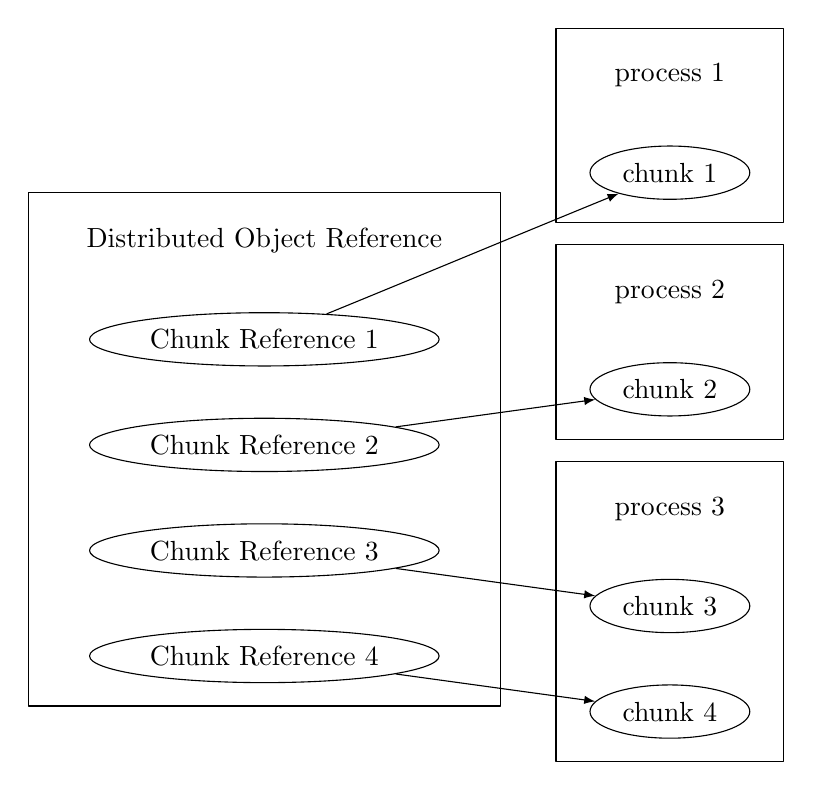
\begin{tikzpicture}[>=latex,line join=bevel,]
%%
\begin{scope}
  \pgfsetstrokecolor{black}
  \definecolor{strokecol}{rgb}{0.0,0.0,0.0};
  \pgfsetstrokecolor{strokecol}
  \draw (0.0bp,28.0bp) -- (0.0bp,213.0bp) -- (170.0bp,213.0bp) -- (170.0bp,28.0bp) -- cycle;
  \draw (85.0bp,195.5bp) node {Distributed Object Reference};
\end{scope}
\begin{scope}
  \pgfsetstrokecolor{black}
  \definecolor{strokecol}{rgb}{0.0,0.0,0.0};
  \pgfsetstrokecolor{strokecol}
  \draw (190.0bp,202.0bp) -- (190.0bp,272.0bp) -- (272.0bp,272.0bp) -- (272.0bp,202.0bp) -- cycle;
  \draw (231.0bp,255.0bp) node {process 1};
\end{scope}
\begin{scope}
  \pgfsetstrokecolor{black}
  \definecolor{strokecol}{rgb}{0.0,0.0,0.0};
  \pgfsetstrokecolor{strokecol}
  \draw (190.0bp,124.0bp) -- (190.0bp,194.0bp) -- (272.0bp,194.0bp) -- (272.0bp,124.0bp) -- cycle;
  \draw (231.0bp,177.0bp) node {process 2};
\end{scope}
\begin{scope}
  \pgfsetstrokecolor{black}
  \definecolor{strokecol}{rgb}{0.0,0.0,0.0};
  \pgfsetstrokecolor{strokecol}
  \draw (190.0bp,8.0bp) -- (190.0bp,116.0bp) -- (272.0bp,116.0bp) -- (272.0bp,8.0bp) -- cycle;
  \draw (231.0bp,99.0bp) node {process 3};
\end{scope}
  \node (cr1) at (85.0bp,160.0bp) [draw,fill=white,ellipse] {Chunk Reference 1};
  \node (cr2) at (85.0bp,122.0bp) [draw,fill=white,ellipse] {Chunk Reference 2};
  \node (cr3) at (85.0bp,84.0bp) [draw,fill=white,ellipse] {Chunk Reference 3};
  \node (cr4) at (85.0bp,46.0bp) [draw,fill=white,ellipse] {Chunk Reference 4};
  \node (c1) at (231.0bp,220.0bp) [draw,fill=white,ellipse] {chunk 1};
  \node (c2) at (231.0bp,142.0bp) [draw,fill=white,ellipse] {chunk 2};
  \node (c3) at (231.0bp,64.0bp) [draw,fill=white,ellipse] {chunk 3};
  \node (c4) at (231.0bp,26.0bp) [draw,fill=white,ellipse] {chunk 4};
  \draw [->] (cr1) ..controls (133.86bp,179.94bp) and (175.11bp,197.13bp)  .. (c1);
  \draw [->] (cr2) ..controls (152.85bp,131.29bp) and (175.38bp,134.41bp)  .. (c2);
  \draw [->] (cr3) ..controls (152.85bp,74.715bp) and (175.38bp,71.586bp)  .. (c3);
  \draw [->] (cr4) ..controls (152.85bp,36.715bp) and (175.38bp,33.586bp)  .. (c4);
%
\end{tikzpicture}


\caption{Distributed object, showing chunks and their references across disparate nodes.}
\label{fig:distobj}
\end{center}
\end{figure}

Communication structure is a further challenge, which has as its answer an implicit virtual topology of the distributed system.
\pkg{largescaler} engages distributed worker nodes in a peer-to-peer fashion, chunks being the core means of addressing, with their location made opaque at the user-level of the system.

Concurrency is an essential component to distributed systems, and this challenge saw its response as both in-process and inter-process concurrency with \pkg{largescaler}; the base supporting layer of the \pkg{largescaler} stack is a bespoke in-memory TCP message queue service that allows for communication between nodes concurrent with their other operations.
Between nodes, routines run asynchronously over chunks, with parallelism implicit and controlled in distributed fashion.

Evaluation and scope serve to speciate languages, as \proglang{R} from \pkg{S}, and they take special forms in a distributed system.
\pkg{largescaler} seeks to minimise any differences from the \proglang{R} language, so as to provide as transparent an experience for developers as possible, but with respect to evaluation, differs in following a call-by-value, as opposed to call-by-need pattern. Furthermore, errors can be caught, but are only propogated to the caller upon emergence of the underlying chunks, with the system favouring asynchrony to strictness. Scope is likewise limited in favour of message transfer efficiency.

In order to enable complex and iterative models, a distributed garbage collection system is also essential.
Such a system should handle mutable underlying chunk data as well.
Mutable data is treated equivalently to immutable data, where all operations on chunks result in new references, with new identifiers, that are surjective to their referent chunks.
\pkg{largescaler} enables garbage collection in an efficient and conservative manner, through automatically keeping track of the directed acyclic graph of chunk generation history alongside each chunk reference, and clearing this upon proof of computation.
Chunks lacking references are marked for deletion and may then be removed by \proglang{R}'s internal garbage collection.

\section{Results}

\pkg{largescaler} serves as a functioning system, capable of performing complex statistical analyses over datasets spanning hundreds of nodes.
The implementation of this system makes use of a layered approach, wherein each layer targets a different category of user.
A description of the implementation structure of \pkg{largescaler} follows.

The system is supported at the base layer by the \pkg{orcv} package, which exists as an in-memory threaded TCP message queue.
It was created specifically for \pkg{largescaler}, making use of the \pkg{C} API for \proglang{R}, though it is sufficiently general to serve the wider purpose of a message queue for the transfer of \proglang{R} objects between \proglang{R} processes.
Central to the functionality of \pkg{orcv} is its multithreaded operation, allowing transfers to take place in the background of the host \proglang{R} process, thereby not blocking computation.
The core userbase of this package is intended as developers on \pkg{largescaler}.

Sitting on top of \pkg{orcv}, the package \pkg{chunknet} enables the creation of detached nodes, which use \pkg{orcv} to communicate, and operate using their own event loops populated via the queue provided by \pkg{orcv}.
The instances of these nodes provided by the package are worker nodes, and a location service, which serve to operate on and locate chunks, respectively.
The client interface is also provided by \pkg{chunknet}, allowing interaction with chunks as the major user-facing class in this package.
Chunks can be interacted with individually, or collected as part of arbitrary-dimension arrays, over which distributed \pkg{apply()}'s and the like are defined.
The main users of this package are intended to be power-users of distributed statistical algorithms who seek to maximise performance.

The package that meets the demanding statistician referenced in Section~\ref{sec:intro} is given by the \pkg{largescaler} package, which offers the distributed object as an abstracted class where chunk distribution is handled implicitly by the package, freeing the statistician to focus on model creation. Further features offered by the package include distributed environment setup, an automatic distributed function converter, distributed functional programming tools such as a reduce operator, distributed i/o, checkpointing, shuffling of datasets with implicit load-balancing, and a \pkg{dplyr} interface to distributed objects.

\section{User Interface}

The \pkg{largescaler} interface is the principal new contribution by this project, delivering a novel means of interacting with distributed data through meaningful primitives defined at every level of abstraction.
A key offering of the layered approach is the ease by which a user of the package can traverse the levels as needed, with irrelevent information remaining hidden until required.
The levels of abstraction correspond to users of the package, given as the following:

\begin{description}
    \item[Analyst] A user solely interested in using the provided models and statistical functions in order to attain insight into some larger-than-memory data, typically a distributed data frame. All details of distribution are abstracted away.
    \item[Researcher] A user seeking to develop their own distributed statistical models. Distributed objects are to be considered as singular cohesive objects.
    \item[Developer] A user seeking greater expressivity in the definition of statistical models. Chunks are considered a relevant concern to be manipulated directly.
    \item[Architect] A user intending to directly modify the network topology of the distributed system, mainly in order to attain major efficiency gains.
\end{description}

Each of the users are served by the aforementioned packages making up the framework.
The main public interface to each package is described in greater detail in the following subsections. 

\subsection{\pkg{largescalemodelr}}

The interface for the analyst, the \pkg{largescalemodelr} public interface consists solely of statistical models.
Beyond the analyst, the source code for the models serve as examples of system usage, and are deliberately styled in such a fashion as to demonstrate the different techniques made possible by the lower layers of the \pkg{largescaler} framework.

Three models are exposed:
\begin{description}
    \item[\texttt{dlm}] Distributed Linear Model
    \item[\texttt{dglm}] Distributed Generalised Linear Model
    \item[\texttt{dlasso}] Distributed LASSO
\end{description}

Each accept distributed objects as arguments for the data sets, with formula interfaces provided for the linear models.

\todo{more in this section?}

\subsection{\pkg{largescaler}}

The framework namesake, \pkg{largescaler} serves to provide a toolbox for the definition of distributed statistical models.
\pkg{largescaler} exposes a range of conceptually related entities

\todo{Distributed Object and methods - [, table, etc.}
\todo{Distributed Object Reference}
\todo{ dplyr}
\todo{ IO}
\todo{ HOF (do.dcall, dreduce \ref{fig:dreduce}, difference w/map-reduce, map-reduce)}
\todo{ checkpoint}
\todo{ combine}
\todo{ cluster initialisation}

\begin{figure}[ht]
\begin{center}
    
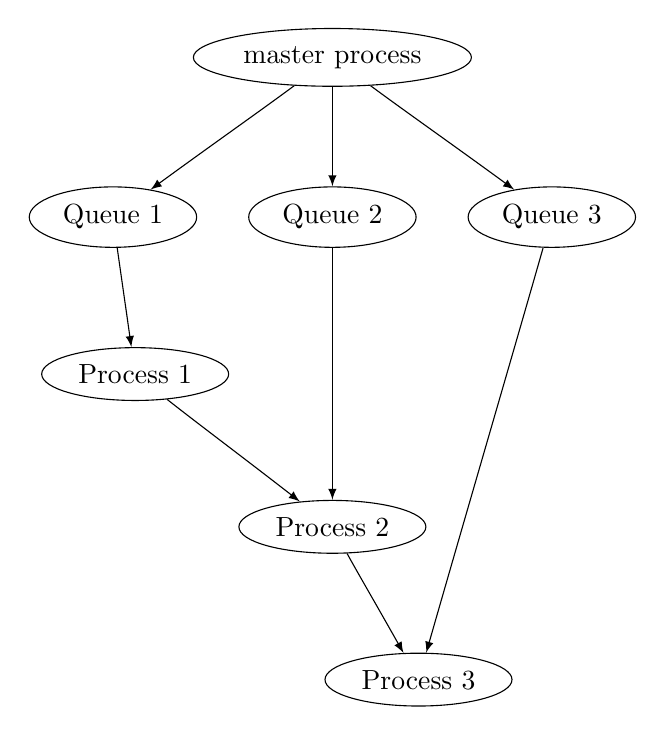
\begin{tikzpicture}[>=latex,line join=bevel,]
%%
\begin{scope}
  \pgfsetstrokecolor{black}
  \definecolor{strokecol}{rgb}{1.0,1.0,1.0};
  \pgfsetstrokecolor{strokecol}
  \definecolor{fillcol}{rgb}{1.0,1.0,1.0};
  \pgfsetfillcolor{fillcol}
  \filldraw (0.0bp,0.0bp) -- (0.0bp,244.0bp) -- (219.0bp,244.0bp) -- (219.0bp,0.0bp) -- cycle;
\end{scope}
\begin{scope}
  \pgfsetstrokecolor{black}
  \definecolor{strokecol}{rgb}{1.0,1.0,1.0};
  \pgfsetstrokecolor{strokecol}
  \definecolor{fillcol}{rgb}{1.0,1.0,1.0};
  \pgfsetfillcolor{fillcol}
  \filldraw (0.0bp,0.0bp) -- (0.0bp,244.0bp) -- (219.0bp,244.0bp) -- (219.0bp,0.0bp) -- cycle;
\end{scope}
  \node (q1) at (30.5bp,176.0bp) [draw,ellipse] {Queue 1};
  \node (q2) at (109.5bp,176.0bp) [draw,ellipse] {Queue 2};
  \node (q3) at (188.5bp,176.0bp) [draw,ellipse] {Queue 3};
  \node (m) at (109.5bp,233.5bp) [draw,ellipse] {master process};
  \node (p1) at (38.5bp,119.5bp) [draw,ellipse] {Process 1};
  \node (p2) at (109.5bp,64.5bp) [draw,ellipse] {Process 2};
  \node (p3) at (140.5bp,9.5bp) [draw,ellipse] {Process 3};
  \draw [->] (m) ..controls (84.261bp,214.77bp) and (65.841bp,201.83bp)  .. (q1);
  \draw [->] (m) ..controls (109.5bp,215.84bp) and (109.5bp,206.15bp)  .. (q2);
  \draw [->] (m) ..controls (134.74bp,214.77bp) and (153.16bp,201.83bp)  .. (q3);
  \draw [->] (q1) ..controls (33.033bp,157.74bp) and (34.506bp,147.71bp)  .. (p1);
  \draw [->] (q2) ..controls (109.5bp,146.51bp) and (109.5bp,107.36bp)  .. (p2);
  \draw [->] (q3) ..controls (177.57bp,137.55bp) and (156.0bp,63.62bp)  .. (p3);
  \draw [->] (p1) ..controls (60.126bp,102.36bp) and (77.076bp,89.704bp)  .. (p2);
  \draw [->] (p2) ..controls (118.86bp,47.493bp) and (125.03bp,36.954bp)  .. (p3);
%
\end{tikzpicture}


\caption{Example distributed reduce pattern from controlling process.}
\label{fig:dreduce}
\end{center}
\end{figure}

\subsection{\pkg{chunknet}}

\subsection{\pkg{orcv}}

\pkg{orcv} is the infrastructure layer that handles the network communications and base node data structures, as an asynchronous communicating event receiver.
This lowest layer is a self-contained package of mostly \proglang{C} descriptions of networking communication and thread-safe internal event queues.
Communications are the core of this package and the main entities given are the listener and receivers.
The listener is simply a standard \lstinline{accept()}er that upon acceptance of a connection passes on the file descriptor to a thread pool of receivers by way of the thread-safe queue.
The receiver that picks up the connection in turn reads from it, passing on whatever message is received to a shared event queue, along with a file descriptor of the connection socket, in order to allow for direct responses to messages.

The two core classes exposed by \pkg{orcv} are the \textsc{Message} and the \textsc{Location} classes, which both seek to abstract some of the more fundamental networking details away.
The \textsc{Message} class captures the notion of the payload, which is sent to some other node given by a \textsc{Location}, using the \lstinline{send()} method.
The payload can be any standard \proglang{R} object.
This is accepted in a separate thread at the receiver location, provided that that the receiver server has been \lstinline{start()}ed, and it is placed on a receiver event queue.
The event queue consists of a basic thread-safe queue, with efficiency gains from \lstinline{poll()}.
The event queue can be popped using a \lstinline{receive()}, and in this fashion communication can take place.

So orcv provides initial network communication capabilities, as well as event queues that can be monitored, with events themselves able to be replied to directly by way of their included file descriptor.
Much of the package structure is related to existing work by \citet{osrv}, with much of the networking architecture taking direct inspiration from \citet{stevens1997network}

\section{Discussion/Conclusions}

The \pkg{largescaler} system has been proven over a number of application areas.
Data manipulation is a basic necessity, as it is required for modelling, and is provided well by other systems.
\pkg{largescaler} is capable of a full set of data manipulations, including all that are provided by the \pkg{dplyr} package.
Model fitting is demonstrated in the proof-of-concept \pkg{largescalemodelr} package, which includes a variety of models, including linear models and generalised linear models.
Work is currently underway to develop examples of boosted models, as well as a convex optimisation methods such as the alternating direction method of multipliers.

Initial benchmarking results are highly promising, with performance results measuring not only speed but capability;
One instance of capability is given in the creation of a contingency table of a large dataset that crashed \proglang{Spark} but was computed in several seconds using \pkg{largescaler}.

The scope for future work remains significant, enabled by the high level of extensibility provided by the system.
External systems which serve to monitor performance or take up the role of garbage collection would grant the possibility of greater reliabilit.
Robustness could be gained through self-healing datasets, a potential that has a precedent in a current prototype, which allows for resiliance to node failure in a more efficient manner than that of the current Resilient Distributed Datasets~\citep{zaharia2012resilient}.
Further resiliance can be gained within the system through operating the location service as a distributed hash table, leaving no central point of failure in a fully peer-to-peer system.

\bibliographystyle{jds}
\bibliography{largescaler-jason-cairns}

\end{document}